\documentclass[english,3p]{elsarticle}

\usepackage[T1]{fontenc}
\usepackage[utf8]{inputenc}
\usepackage{babel}
\usepackage{color}
\usepackage[usenames,dvipsnames]{xcolor}
\usepackage{bm}
\usepackage{setspace}
\usepackage{amssymb}
\usepackage{amsmath}
\usepackage{amsfonts}

\newcommand{\todo}[1]{\colorbox{yellow}{\textbf{#1}}}
\newcommand{\code}[1]{\texttt{#1}}
\newcommand{\ii}{\mathrm{i}}
\newcommand{\ee}{\mathrm{e}}
\newcommand{\dd}{\mathrm{d}}

\usepackage{listings}
\usepackage{color}

\definecolor{mygreen}{rgb}{0,0.6,0}
\definecolor{mygray}{rgb}{0.5,0.5,0.5}
\definecolor{mymauve}{rgb}{0.58,0,0.82}

\lstdefinestyle{customc}{
  belowcaptionskip=1\baselineskip,
  breaklines=true,
  frame=l,
  xleftmargin=\parindent,
  language=C,
  showstringspaces=false,
  basicstyle=\footnotesize\ttfamily,
  keywordstyle=\bfseries\color{green!40!black},
  commentstyle=\itshape\color{purple!40!black},
  identifierstyle=\color{blue},
  stringstyle=\color{orange},
}
\lstdefinestyle{customasm}{
  belowcaptionskip=1\baselineskip,
  frame=L,
  xleftmargin=\parindent,
  language=[x86masm]Assembler,
  basicstyle=\footnotesize\ttfamily,
  commentstyle=\itshape\color{purple!40!black},
}
\lstset{escapechar=@,style=customc}

\begin{document}

\begin{center}
EAA Winter School in Computational Acoustics

Le Mans Université, December 2018
\vspace{5mm}

\textbf{\large Tutorial on FreeFEM++}
\end{center}

\vspace{10mm}

This part of the tutorial on finite elements uses the FreeFEM++ package which is freely available at \texttt{https://freefem.org}.
The documentation can be found at \texttt{https://doc.freefem.org}.
It is already installed on the workstations.
To use it you can...

\section{Sound field in a cavity}

We begin with the calculation of the sound field in a cavity with a vibrating wall.
This sound field is governed by the Helmholtz equation
\begin{equation}
k^2p + \nabla^2 p = 0
\;,
\label{eq:helmholtz}
\end{equation}
where $k=\omega/c_0$ is the acoustic wavenumber with $\omega$ the angular frequency and $c_0$ the sound speed.

The first part of the file \code{cavity.edp} defines a number of boundaries for the computational domain shown in figure \ref{fig:CavityGeometry}:
\begin{figure}[h]
\centering
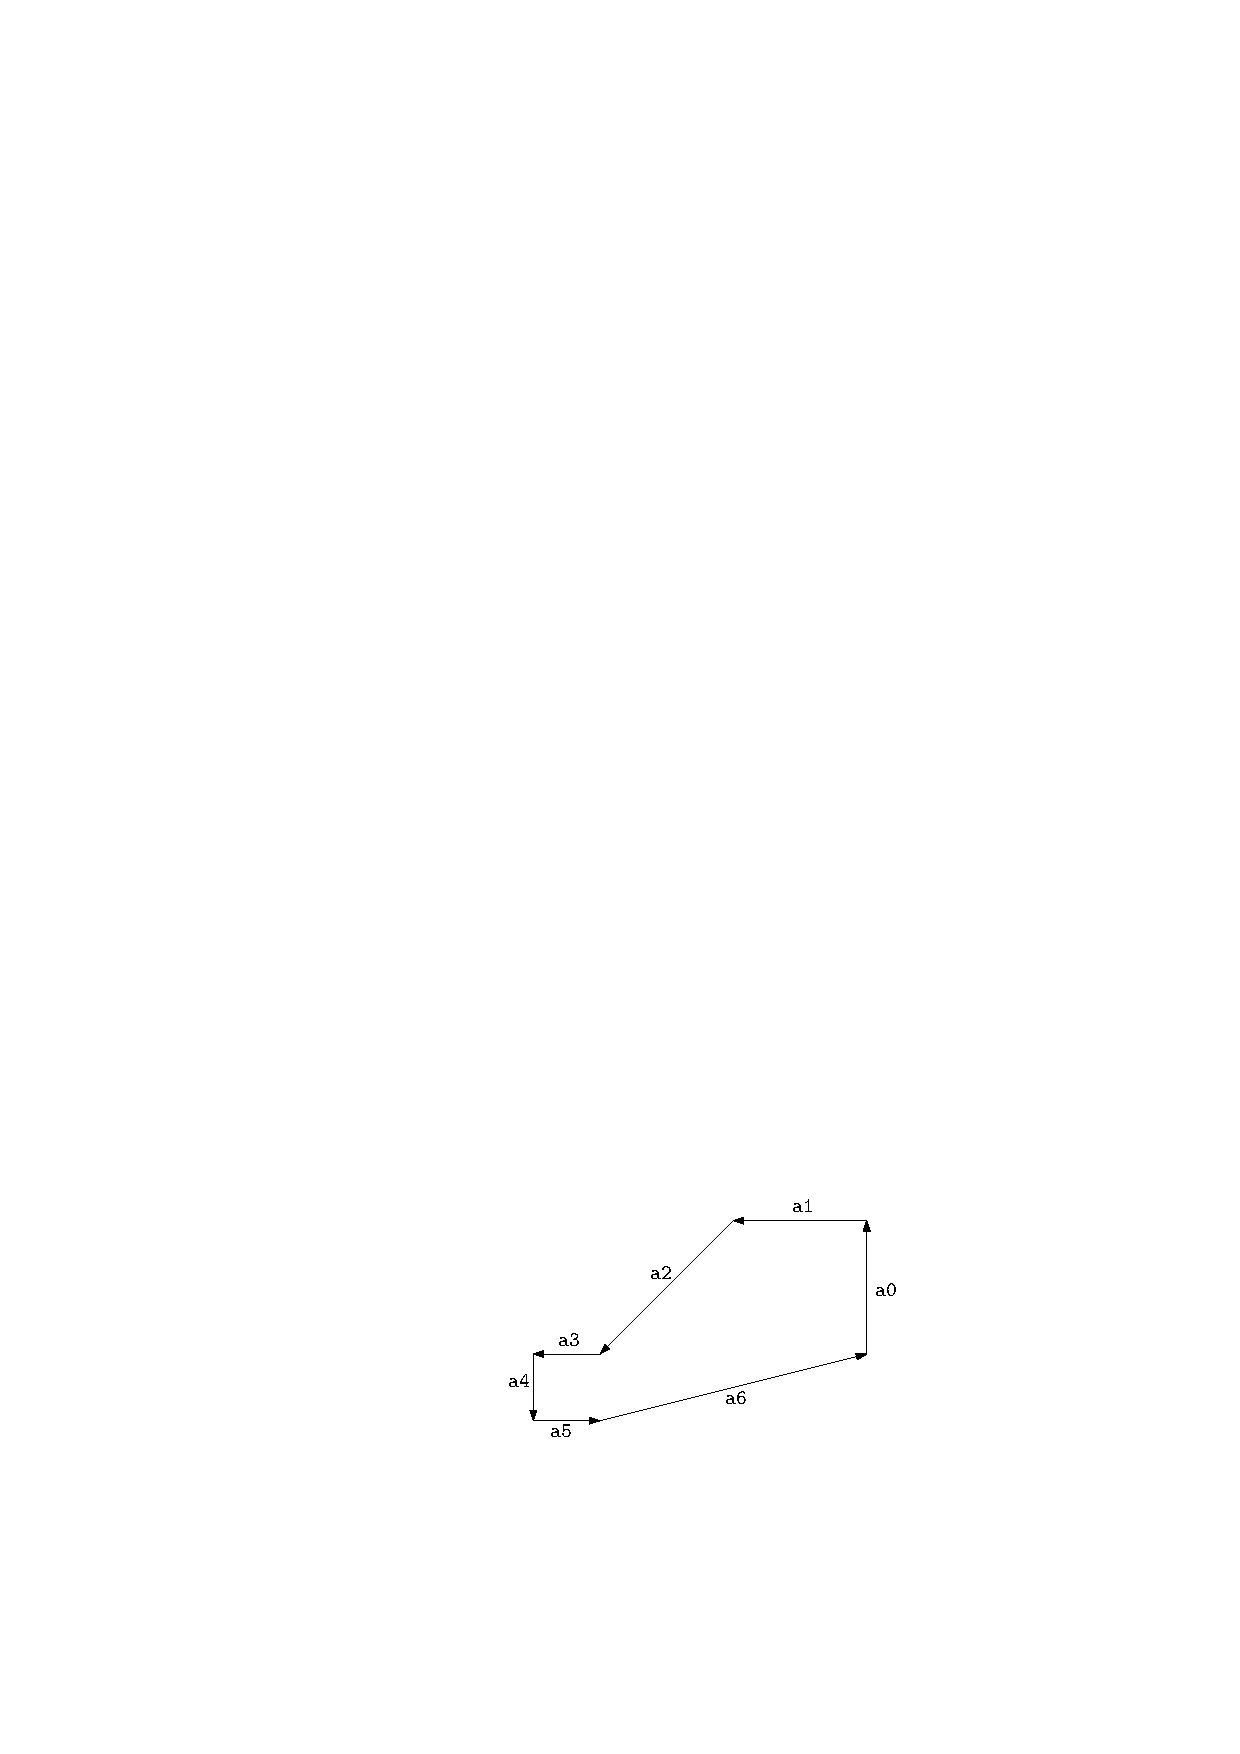
\includegraphics[width=60mm]{cavity.pdf}
\hfill
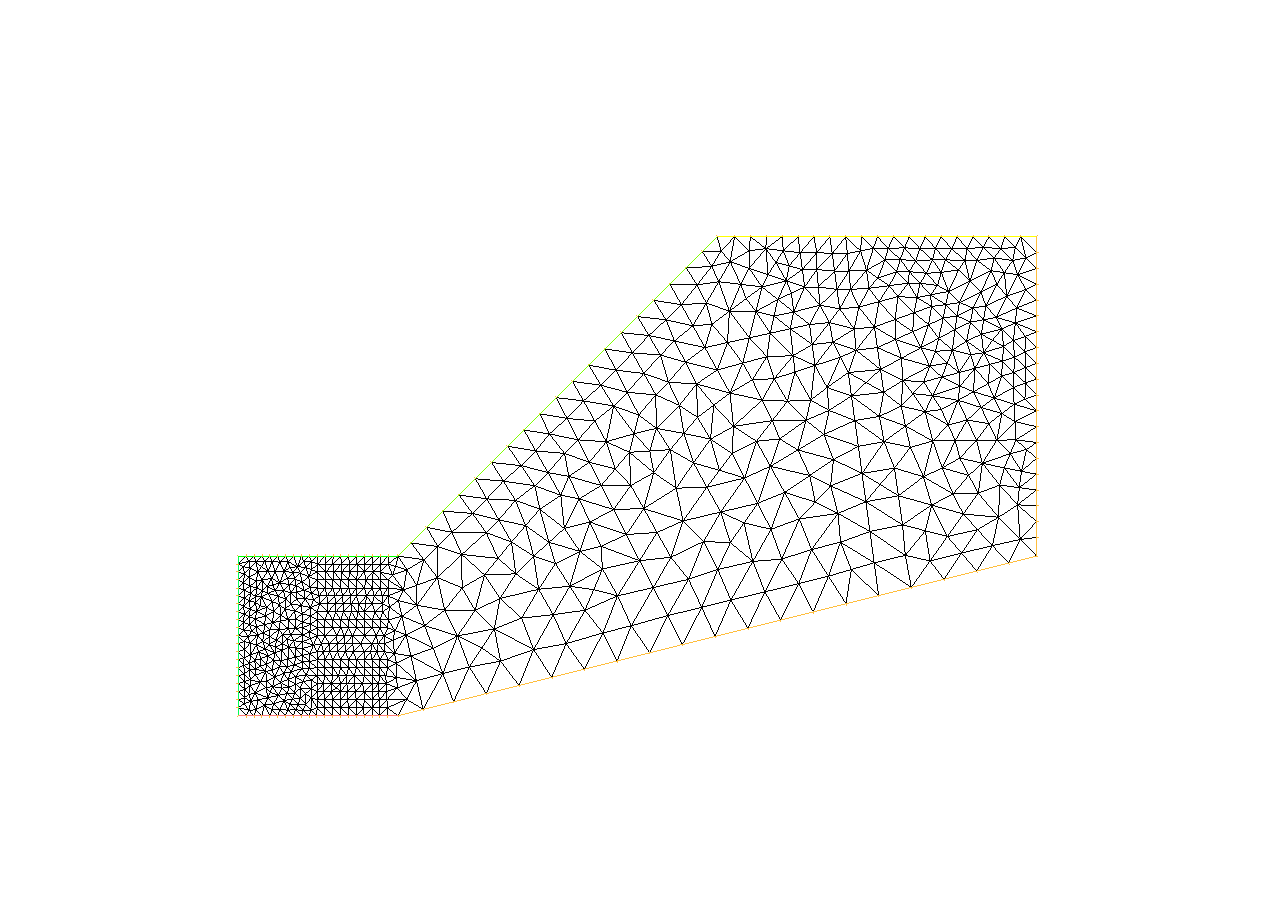
\includegraphics[width=80mm]{mesh.eps}
\caption{Left: Geometry of the computational domain; Right: Example of triangular mesh for the cavity.}
\label{fig:CavityGeometry}
\end{figure}
\begin{lstlisting}
// Create the boundaries of the computational domain
border a0(t=0,1) { x= 5; y= 1+2*t ;}
border a1(t=0,1) { x=5-2*t; y= 3 ;} 
border a2(t=0,1) { x= 3-2*t; y=3-2*t ;}
border a3(t=0,1) { x= 1-t; y= 1 ;} 
border a4(t=0,1) { x= 0; y= 1-t ;} 
border a5(t=0,1) { x= t; y= 0 ;} 
border a6(t=0,1) { x= 1+4*t; y= t ;}
\end{lstlisting}
Each boundary is parametrized using a parameter \code{t} varying from 0 to 1.

The next step is to generate a mesh of the computational domain using triangular elements and 20 elements per boundary:
\begin{lstlisting}
// Generate a mesh of the domain using 20 elements per edge
mesh Th=buildmesh( a0(20) + a1(20) + a2(20) + a3(20) + a4(20) + a5(20) + a6(20) );
\end{lstlisting}
The resulting mesh can then be shown using the following command, see figure \ref{fig:CavityGeometry}.
\begin{lstlisting}
// Plot the mesh
plot(Th, wait=1, ps="Th.eps");
\end{lstlisting}

We define the approximation space \code{Vh} which is formed of linear interpolation functions (\code{P1} denotes the polynomials of order 1) on the mesh \code{Th} previously created:
\begin{lstlisting}
// Define the approximation space based on linear elements
fespace Vh(Th,P1);
Vh p,q;
\end{lstlisting}

Finally we can solve the following variational formulation for the Helmholtz equation where we impose $\partial p/\partial n=1$ on the boundary $\Gamma_4$:
$$
\int_\Omega k^2qp - \nabla q\cdot\nabla p\,\dd\Omega+
\int_{\Gamma_4} q\,\dd\Gamma
=0
\;,\quad
\forall q
\;.
$$
\begin{lstlisting}
// Solve the variational formulation for the Helmholtz equation
real k = 10;
solve cavity(p,q)=int2d(Th)(k*k*p*q - dx(p)*dx(q) - dy(p)*dy(q)) - int1d(Th,a4)(q);
\end{lstlisting}
In this code we solve the problem for a wavenumber $k=10$.

We can plot the pressure field given by the finite-element model:
\begin{lstlisting}
// Plot the result
plot(p, fill=1);
\end{lstlisting}
which gives figure \ref{fig:solution1}.
\begin{figure}[h]
\centering
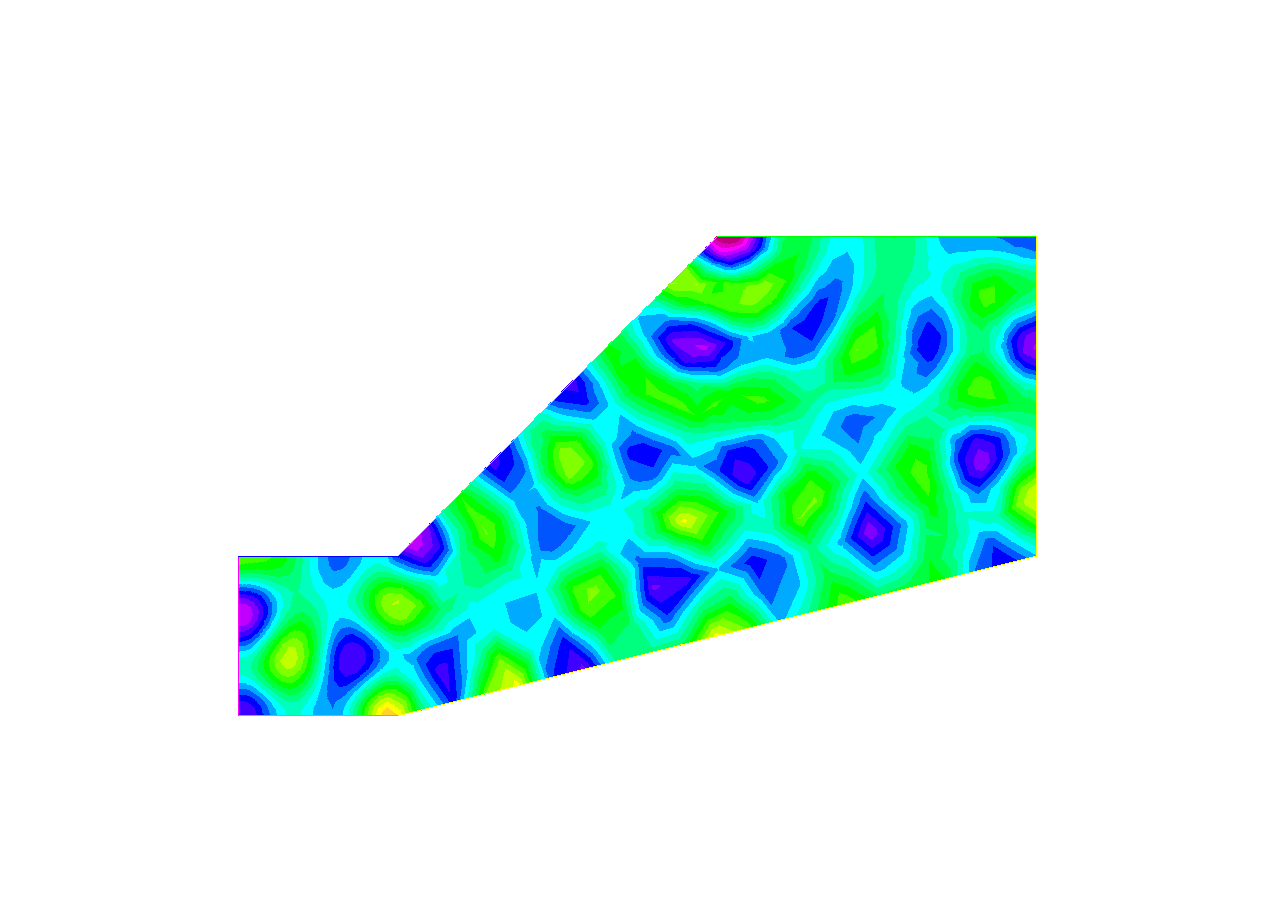
\includegraphics[width=80mm]{solution_P1.eps}
\caption{Solution of the cavity problem using linear elements and 20 elements per boundary.}
\label{fig:solution1}
\end{figure}

\textbf{Question 1:} Switch to a quadratic approximation space by using \code{P2} instead of \code{P1} in the definition of the approximation space \code{Vh}.

\textbf{Question 2:} Using a linear approximation of the solution, use a finer mesh with 40 element along each boundary.
For $k=10$, how many elements per wavelength does this correspond to?

\textbf{Question 3:} Of the two solutions produced in the previous two questions which one appears the more accurate? Why?

\textbf{Question 4:} Change the variational formulation in the file \code{cavity.edp} so that the forcing is applied on the boundary $\Gamma_6$.

\clearpage

\section{Modes of vibration of a tuning fork}

The second example we consider is the modes of vibration of a tuning fork in two dimensions.
The geometry of the fork is shown in figure \ref{fig:mesh_fork}.
The vibration of the tuning fork follows the equation of linear elasticity in the time-harmonic regime (with a time dependence $\ee^{\ii\omega t}$):
\begin{equation}
-\rho\omega^2\mathbf{u} = \nabla\cdot\boldsymbol{\sigma}
\;,\quad
\boldsymbol{\sigma}(\mathbf{u}) = \lambda\nabla\cdot\mathbf{u} + 2\mu\boldsymbol{\varepsilon}
\;,\quad
\boldsymbol{\varepsilon}(\mathbf{u}) = \frac{1}{2}( \nabla\mathbf{u} + \nabla\mathbf{u}^T )
\;,
\label{eq:elasticity}
\end{equation}
where $\mathbf{u}$ is the displacement of the elastic solid, $\boldsymbol{\sigma}$ is the stress tensor and $\boldsymbol{\varepsilon}$ is the strain tensor.
$\lambda$ and $\mu$ are the Lamé coefficients and $\rho$ is the material density.
The boundary conditions on the tuning fork are that there is no normal stress on the surface ($\boldsymbol{\sigma}\cdot\mathbf{n} = 0$) except at the base of the fork (denoted $\Gamma_2$) where it is fixed ($\mathbf{u}=\mathbf{0}$).

The input file to solve this problem with FreeFEM++ is called \code{tuning\_fork.edp}.
Please read through the comments included in this file.
After generating a mesh of the tuning fork (see figure \ref{fig:mesh_fork}), the script calculates the mass and stiffness matrices based on the following variational formulation:
$$
\int_\Omega \boldsymbol{\sigma}(\mathbf{u}):\boldsymbol{\varepsilon}(\mathbf{v}) - \rho\omega^2\mathbf{u}\cdot\mathbf{v}\,\dd\Omega
\;,\quad
\text{with } \mathbf{u}=\mathbf{0} \text{ on } \Gamma_2
\;,\quad
\forall \mathbf{v}
\;,
$$
where $\mathbf{v}$ is the test function associated with the displacement field $\mathbf{u}$.
An eigenvalue problem is then solved to find the resonance frequencies $\omega$ of the tuning fork as well as the associated displacement fields.
The deformed shape of the tuning fork induced by each mode is shown in turn.
The resonance frequencies of the modes are also printed out.

\begin{figure}[h]
\centering
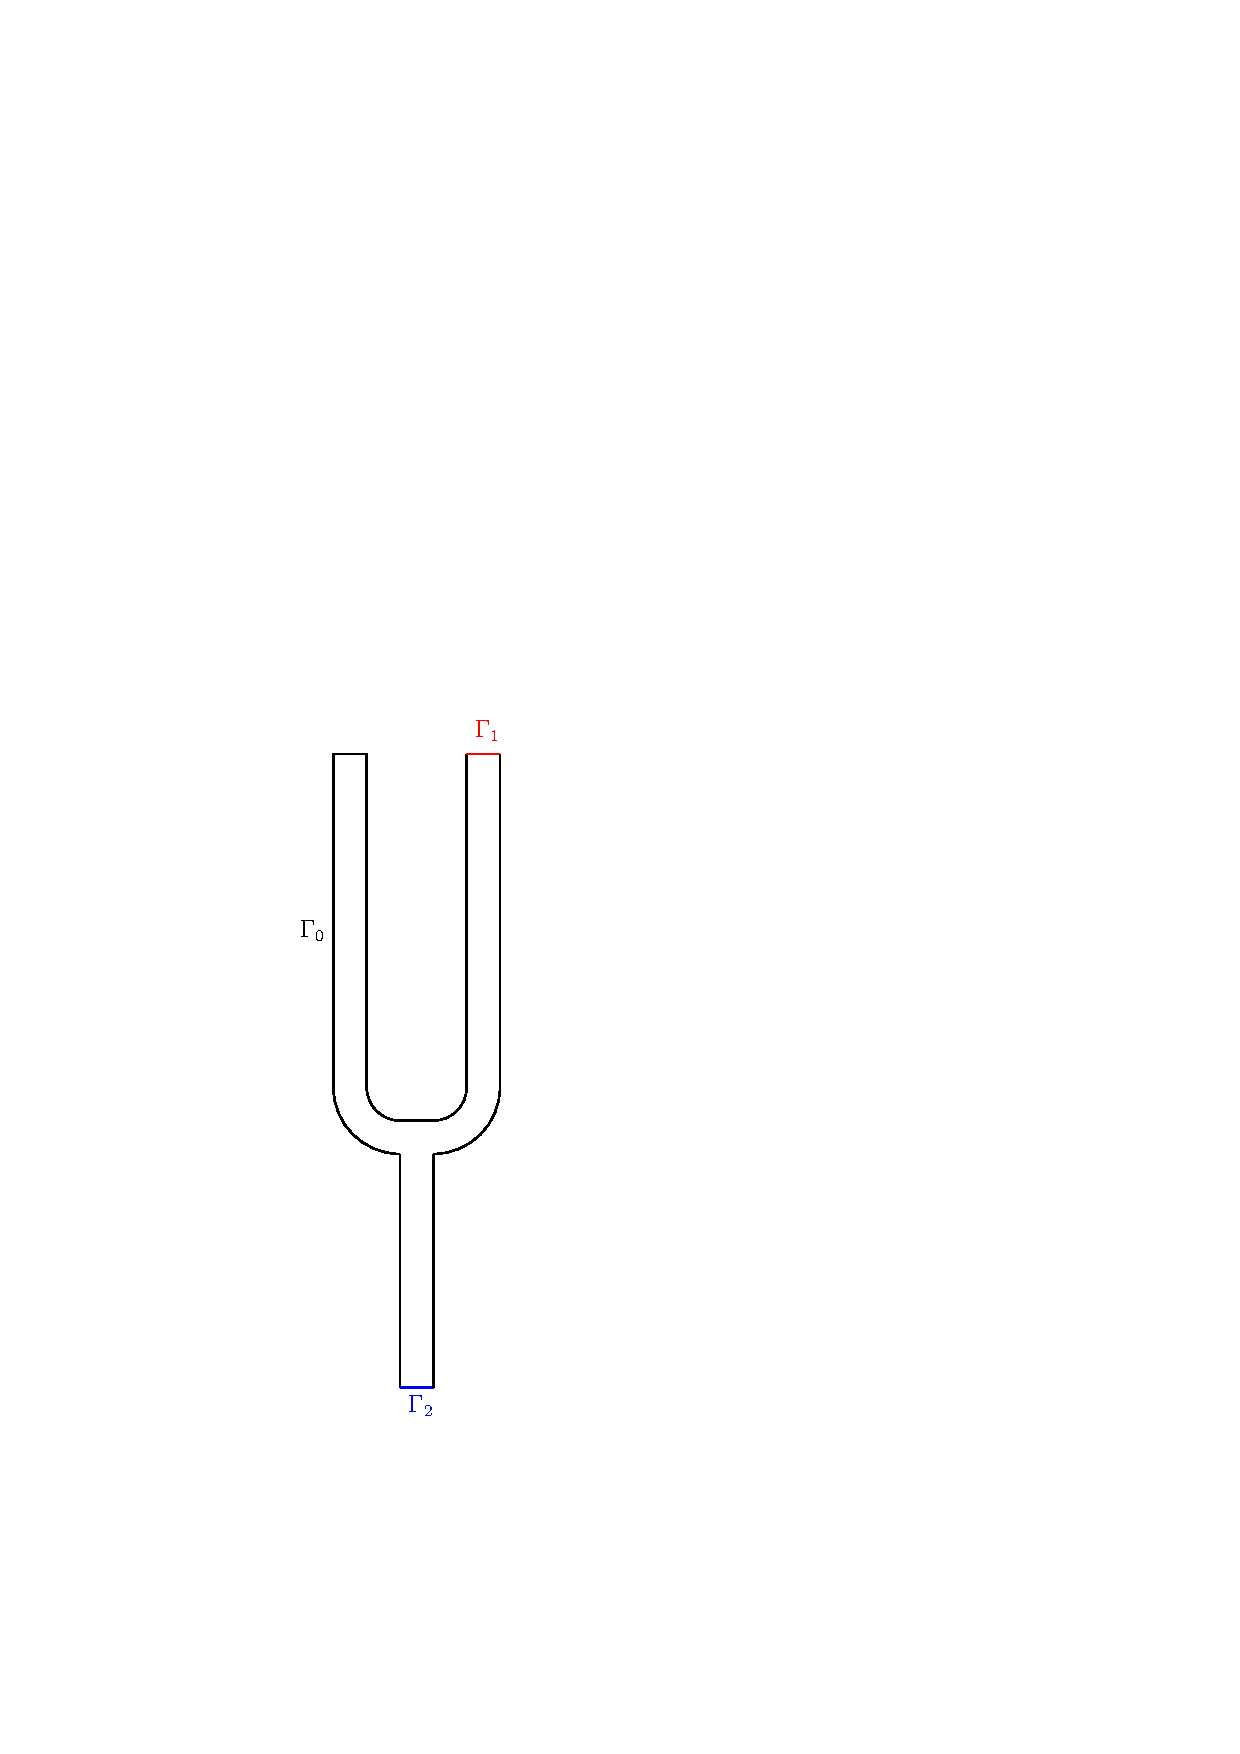
\includegraphics[width=17mm]{fork.pdf}
\hspace{20mm}
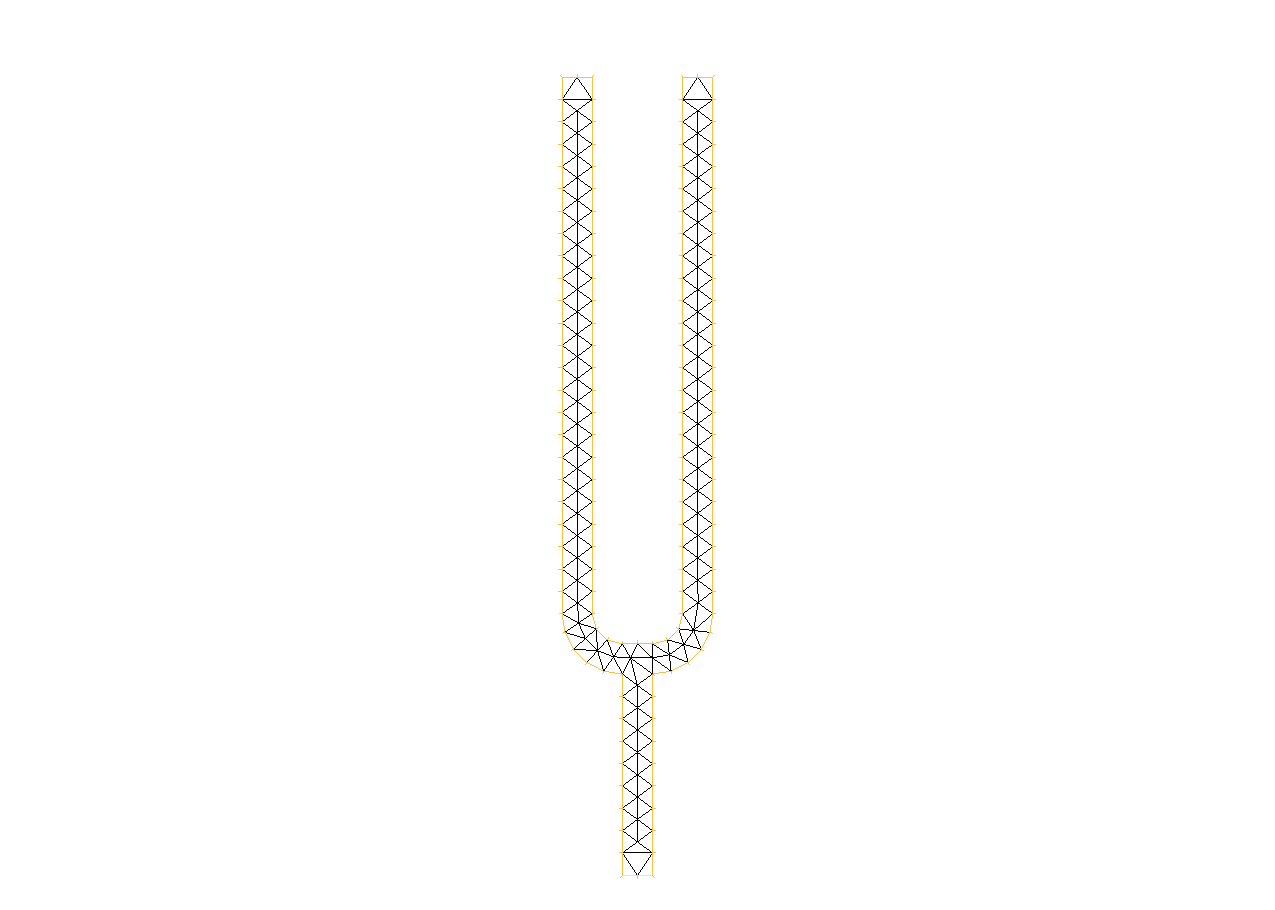
\includegraphics[width=80mm]{fork_mesh.eps}
\caption{Left: Geometry of the computational domain. Right: Mesh for the tuning fork.}
\label{fig:mesh_fork}
\end{figure}

\textbf{Question 5:} Increase the mesh resolution by changing the variable \code{nbe} and see how this influences the resonance frequencies.

\clearpage

\section{Fluid-structure interaction}

In this section we still consider the tuning fork but we now include the coupling between the fork and the surrounding air, and we calculate the response of these coupled systems (fluid \& structure) to a time-harmonic excitation.

The equations of motion for the structure are those given in equation \eqref{eq:elasticity}.
The sound waves in the fluid surrounding the tuning fork are governed by the Helmholtz equation \eqref{eq:helmholtz}.
The variational formulations are as follows:
$$
\int_{\Omega_\mathrm{s}} \boldsymbol{\sigma}(\mathbf{u}):\boldsymbol{\varepsilon}(\mathbf{v}) - \rho\omega^2\mathbf{u}\cdot\mathbf{v}\,\dd\Omega - \int_{\Gamma_0} p \mathbf{v}\cdot\mathbf{n}_\mathrm{s}\,\dd\Gamma
-\int_{\Gamma_1} \mathbf{v}\cdot\mathbf{t}\,\dd\Gamma
\;,\quad
\text{with } \mathbf{u}=\mathbf{0} \text{ on } \Gamma_2
\;,\quad
\forall \mathbf{v}
$$
$$
\frac{1}{\rho_0\omega^2}\int_{\Omega_\mathrm{a}} \nabla q\cdot\nabla p - k^2qp \,\dd\Omega - \int_{\Gamma_0} q\mathbf{u}\cdot\mathbf{n}_\mathrm{a}\,\dd\Gamma
=0
\;,\quad
\forall q
\;.
$$
$\Omega_\mathrm{s}$ and $\Omega_\mathrm{a}$ are the structure and fluid domains, respectively.
$\mathbf{t}$ is the force on the fork on its upper right boundary ($\Gamma_1$).
The last terms in each of these equations are responsible for the coupling between the fluid and the structure.

\textbf{Question 6:} ...

\textbf{Question 7:} ...

\textbf{Question 8:} ...

\end{document}
